% Options for packages loaded elsewhere
\PassOptionsToPackage{unicode}{hyperref}
\PassOptionsToPackage{hyphens}{url}
%
\documentclass[
]{article}
\usepackage{amsmath,amssymb}
\usepackage{lmodern}
\usepackage{iftex}
\ifPDFTeX
  \usepackage[T1]{fontenc}
  \usepackage[utf8]{inputenc}
  \usepackage{textcomp} % provide euro and other symbols
\else % if luatex or xetex
  \usepackage{unicode-math}
  \defaultfontfeatures{Scale=MatchLowercase}
  \defaultfontfeatures[\rmfamily]{Ligatures=TeX,Scale=1}
\fi
% Use upquote if available, for straight quotes in verbatim environments
\IfFileExists{upquote.sty}{\usepackage{upquote}}{}
\IfFileExists{microtype.sty}{% use microtype if available
  \usepackage[]{microtype}
  \UseMicrotypeSet[protrusion]{basicmath} % disable protrusion for tt fonts
}{}
\makeatletter
\@ifundefined{KOMAClassName}{% if non-KOMA class
  \IfFileExists{parskip.sty}{%
    \usepackage{parskip}
  }{% else
    \setlength{\parindent}{0pt}
    \setlength{\parskip}{6pt plus 2pt minus 1pt}}
}{% if KOMA class
  \KOMAoptions{parskip=half}}
\makeatother
\usepackage{xcolor}
\usepackage[margin=1in]{geometry}
\usepackage{graphicx}
\makeatletter
\def\maxwidth{\ifdim\Gin@nat@width>\linewidth\linewidth\else\Gin@nat@width\fi}
\def\maxheight{\ifdim\Gin@nat@height>\textheight\textheight\else\Gin@nat@height\fi}
\makeatother
% Scale images if necessary, so that they will not overflow the page
% margins by default, and it is still possible to overwrite the defaults
% using explicit options in \includegraphics[width, height, ...]{}
\setkeys{Gin}{width=\maxwidth,height=\maxheight,keepaspectratio}
% Set default figure placement to htbp
\makeatletter
\def\fps@figure{htbp}
\makeatother
\setlength{\emergencystretch}{3em} % prevent overfull lines
\providecommand{\tightlist}{%
  \setlength{\itemsep}{0pt}\setlength{\parskip}{0pt}}
\setcounter{secnumdepth}{5}
\RequirePackage{amsthm,amsmath,amsfonts,amssymb}
\RequirePackage[authoryear]{natbib}
\RequirePackage{bm}
\RequirePackage{enumerate}
\RequirePackage{enumitem}
\RequirePackage{tabularx}
\RequirePackage{adjustbox}
\RequirePackage{tikz}
\RequirePackage{bbm}
\RequirePackage{lscape}
\RequirePackage{booktabs}
\RequirePackage{longtable}
\RequirePackage{lscape}
\RequirePackage{pifont}
\usepackage{footnote}

\newcommand{\Sc}{\mathcal{S}}
\newcommand{\R}{\mathcal{R}}
\newcommand{\N}{\mathcal{N}}
\newcommand{\X}{\mathcal{X}}
\newcommand{\m}{\mathbf{m}}
\newcommand{\bu}{\mathbf{u}}
\newcommand{\bv}{\mathbf{v}}
\newcommand{\w}{\mathbf{w}}
\newcommand{\x}{\mathbf{x}}
\newcommand{\y}{\mathbf{y}}
\newcommand{\z}{\mathbf{z}}
\newcommand{\bb}{\mathbf{b}}
\newcommand{\brho}{\bm{\rho}}
\newcommand{\bphi}{\bm{\phi}}
\newcommand{\btheta}{\bm{\theta}}
\newcommand{\bpsi}{\bm{\psi}}

\newcommand{\cmark}{\ding{51}}
\newcommand{\xmark}{\ding{55}}

\usepackage{amsmath}
\DeclareMathOperator*{\argmin}{arg\,min}
\ifLuaTeX
  \usepackage{selnolig}  % disable illegal ligatures
\fi
\IfFileExists{bookmark.sty}{\usepackage{bookmark}}{\usepackage{hyperref}}
\IfFileExists{xurl.sty}{\usepackage{xurl}}{} % add URL line breaks if available
\urlstyle{same} % disable monospaced font for URLs
\hypersetup{
  pdftitle={Understanding the eradication of malaria in the United States 1920-1950},
  hidelinks,
  pdfcreator={LaTeX via pandoc}}

\title{Understanding the eradication of malaria in the United States
1920-1950}
\usepackage{etoolbox}
\makeatletter
\providecommand{\subtitle}[1]{% add subtitle to \maketitle
  \apptocmd{\@title}{\par {\large #1 \par}}{}{}
}
\makeatother
\subtitle{Adam Howes (\texttt{ath19@ic.ac.uk})}
\author{}
\date{\vspace{-2.5em}}

\begin{document}
\maketitle

\hypertarget{background}{%
\section{Background}\label{background}}

\begin{itemize}
\tightlist
\item
  Malaria eradicated in the US during the years 1920-1950
\item
  Interest in learning why this happened, or which factors were
  associated with faster eradication
\item
  Have county level malaria data from various sources, with some
  limiations
\item
  Have county level covariate data form various sources, with some
  limitations
\end{itemize}

\hypertarget{data}{%
\section{Data}\label{data}}

\begin{itemize}
\tightlist
\item
  Malaria data as follows\ldots{}
\item
  Covariate data in the following categories

  \begin{itemize}
  \tightlist
  \item
    County
  \item
    Drainage
  \item
    Farmland
  \item
    Mortality
  \item
    People
  \item
    Socioeconomic
  \item
    Weather
  \item
    Zooprophylaxis
  \end{itemize}
\end{itemize}

\hypertarget{model}{%
\section{Model}\label{model}}

\begin{itemize}
\tightlist
\item
  As implemented in \texttt{fit\_sae-Y20-50}
\item
  Uses \texttt{malariadata.csv} and \texttt{southern13\_areas.geojson}
\item
  Calculates mortality rate per 100,000
\item
  For categorical data, takes some single fixed numeric value.

  \begin{itemize}
  \tightlist
  \item
    This could be improved using imputation via fitting a model, which I
    have started in \texttt{impute\_numeric-Y33-37} but not finished
  \end{itemize}
\item
  Model defined for all years 1920 to 1950, and the counties from
  \texttt{southern13\_areas.geojson}
\item
  For covariates not available in a particular year and county, I
  imputed using \texttt{missForest()} and normalised the output (see
  \texttt{impute\_covariates})

  \begin{itemize}
  \tightlist
  \item
    I don't think the imputed covariates are good. Just looking at the
    time series output you get it's not what you'd want
  \end{itemize}
\item
  Model formula uses a fixed effect for each covariate, a Besag model on
  space at the country level, and an AR1 model on time at the year level
\item
  Use a Poisson likelihood adapted to account for non-integer counts
\item
  Fit the model with the \texttt{R-INLA} implementation of INLA
\end{itemize}

\hypertarget{results}{%
\section{Results}\label{results}}

\begin{itemize}
\tightlist
\item
  Generate plausible seeming posterior means at a state level
\item
  Don't particularly like the way that the data for 1933-1937 is handled
\item
  Strange upswing at the end of the time period where there is no data
\item
  Generate estimates of association with malaria rate of the covariates

  \begin{itemize}
  \tightlist
  \item
    Only association, no causation
  \item
    Covariate inputation algorithm I don't think is good
  \item
    Perhaps they're of interest anyway, I'm not sure
  \end{itemize}
\end{itemize}

\begin{figure}

{\centering 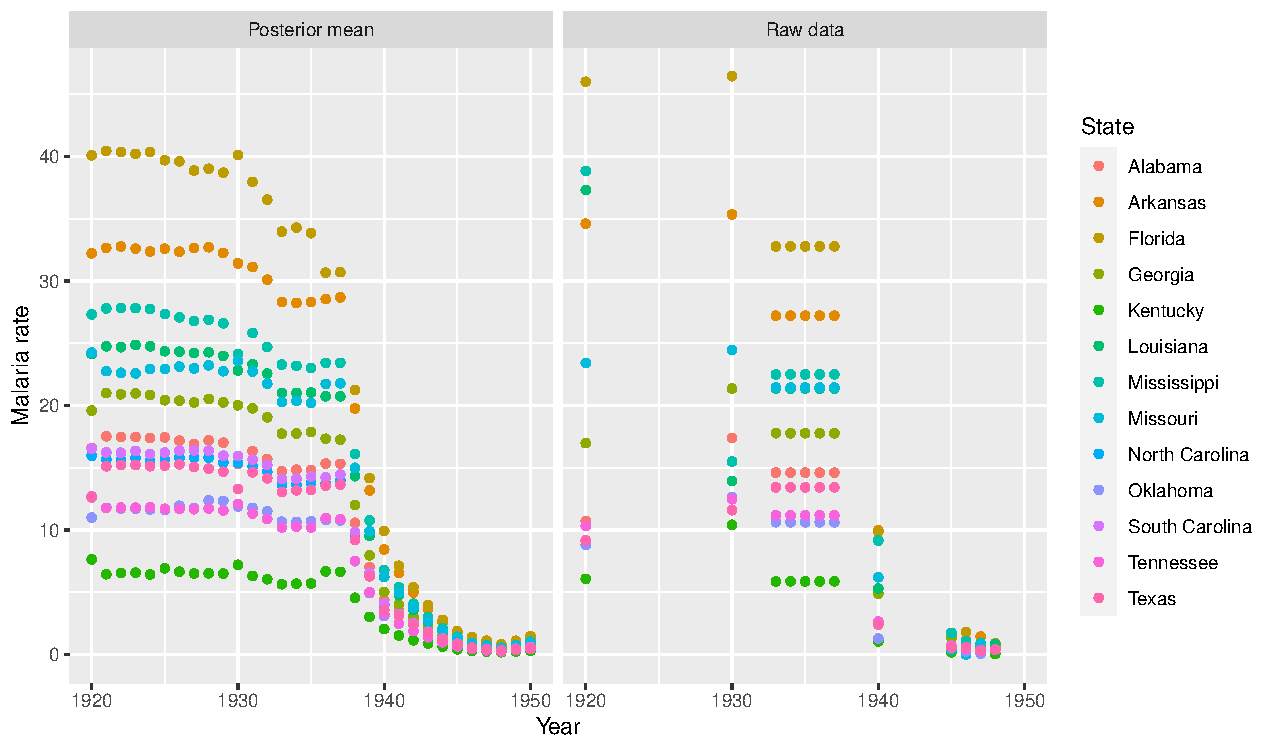
\includegraphics[width=0.95\linewidth]{depends/time-series-state} 

}

\caption{Posterior mean of malaria rate at a state level as compared with the raw data.}\label{fig:unnamed-chunk-2}
\end{figure}

\begin{figure}

{\centering \includegraphics[width=0.95\linewidth]{depends/covariate-imporance} 

}

\caption{Posterior mean and credible intervals for regression coefficient parameters for each covariate.}\label{fig:unnamed-chunk-3}
\end{figure}

\end{document}
